\documentclass[12pt]{article}

\title{Lab Assignment 3}
\author{Cameron Mattson}

% import a set of useful packages for math
\usepackage{amsmath, amsfonts, amssymb}
\usepackage{tcolorbox}
\usepackage{multirow}

% this package makes margins smaller
\usepackage{fullpage}
\usepackage{listings}
\usepackage{amsmath}
\usepackage{graphicx}
\usepackage{listing}
% for importing images
%%%%%%%%%%%%%%%%%%%%%%%%%%%%%%%%
\begin{document}
\maketitle
\tableofcontents

\section{Impact of RNN Architecture}
\subsection{Code}
\begin{lstlisting}[breaklines]
import os
from keras.layers import TextVectorization
from sklearn.model_selection import train_test_split
import tensorflow as tf
import numpy as np
from keras.layers import Embedding
from keras.initializers import Constant
from keras.models import Sequential
from keras.layers import Dense, Dropout, LSTM
from keras.callbacks import ModelCheckpoint
from tensorflow.keras.utils import to_categorical
from keras import layers, Input, Model
from sklearn.metrics import precision_score, recall_score

X_pathneg = 'rt-polarity.neg'
X_pathpos = 'rt-polarity.pos'

with open(X_pathneg, encoding = "ISO-8859-1") as file:
    X_listneg = file.readlines()

with open(X_pathpos, encoding = "ISO-8859-1") as file:
    X_listpos = file.readlines()
 
X_list = X_listneg + X_listpos
y_list = [0]*len(X_listneg) + [1]*len(X_listpos)

X_list = [classval[:-1] for classval in X_list]
classes = np.unique(y_list)
unique_letters = np.unique(X_list)

embed_dim = 100
vectorizer = TextVectorization(max_tokens=20600, output_sequence_length=embed_dim)
text_ds = tf.data.Dataset.from_tensor_slices(X_list).batch(128) ## Read batches of 128 samples
vectorizer.adapt(text_ds)

vocab = vectorizer.get_vocabulary()
vocab_to_index = dict(zip(vocab,range(len(vocab))))
index_to_vocab = dict(zip(range(len(vocab)),vocab))

X_train, X_test, y_train, y_test = train_test_split(X_list, y_list, train_size = 7/10, random_state = 1)

X_train = vectorizer(np.array([[s] for s in X_train])).numpy()
X_test = vectorizer(np.array([[s] for s in X_test])).numpy()

y_train = to_categorical(y_train).astype(np.int64)
y_test = to_categorical(y_test).astype(np.int64)
y_test_labels = np.argmax(y_test, axis = 1)

words_per_sen = np.count_nonzero(X_test, axis = 1)
pertile = np.array([np.percentile(words_per_sen,(1/3*100)), np.percentile(words_per_sen,(2/3*100))])

shortind = np.nonzero(words_per_sen <= pertile[0])[0]
mediumind = np.nonzero(np.logical_and(words_per_sen >= pertile[0], words_per_sen <= pertile[1]))[0]
longind = np.nonzero(words_per_sen > pertile[1])[0]

shortlist = [X_test[shortind,:], y_test[shortind,:], np.argmax(y_test[shortind,:], axis = 1)]
mediumlist = [X_test[mediumind,:], y_test[mediumind,:], np.argmax(y_test[mediumind,:], axis = 1)]
longlist = [X_test[longind,:], y_test[longind,:], np.argmax(y_test[longind,:], axis = 1)]

class models:

  def __init__(self, xtrain, ytrain, embed_layer):
    self.X_train = xtrain
    self.y_train = ytrain
    self.embedding_layer = embed_layer
    self.modmetrics = []

  def get_metrics(self,ytest,ypred):
    self.modmetrics.append([precision_score(ytest, ypred), recall_score(ytest, ypred)])
    return self

  def get_pred(self, X_test, y_test):
    modpreds = np.argmax(self.savedmodel.predict(X_test), axis = 1)
    y_test = np.argmax(y_test, axis = 1)
    self.get_metrics(y_test,modpreds)
    self.y_pred = modpreds
    return self

  def lstm_mod(self):
    classes = self.y_train.shape[1]
    int_sequences_input = Input(shape=(None,), dtype="int64")
    embedded_sequences = self.embedding_layer(int_sequences_input)
    x = layers.Bidirectional(layers.LSTM(20))(embedded_sequences)
    preds = layers.Dense(classes, activation="softmax")(x)
    model1 = Model(int_sequences_input, preds)
    #model1.summary()

    model1.compile(loss="categorical_crossentropy", optimizer="adam")
    model1.fit(self.X_train, self.y_train, batch_size=128, epochs=2)
    
    self.savedmodel = model1

    return self

  def gru_mod(self):
    classes = self.y_train.shape[1]    
    int_sequences_input = Input(shape=(None,), dtype="int64")
    embedded_sequences = self.embedding_layer(int_sequences_input)
    x = layers.Bidirectional(layers.GRU(20))(embedded_sequences)
    preds = layers.Dense(classes, activation="softmax")(x)
    model2 = Model(int_sequences_input, preds)
    #model2.summary()

    model2.compile(loss="categorical_crossentropy", optimizer="adam")
    model2.fit(self.X_train, self.y_train, batch_size=128, epochs=2)
    
    self.savedmodel = model2

    return self

  def rnn_mod(self):
    classes = self.y_train.shape[1]
    int_sequences_input = Input(shape=(None,), dtype="int64")
    embedded_sequences = self.embedding_layer(int_sequences_input)
    x = layers.Bidirectional(layers.SimpleRNN(20))(embedded_sequences)
    preds = layers.Dense(classes, activation="softmax")(x)
    model3 = Model(int_sequences_input, preds)
    #model3.summary()

    model3.compile(loss="categorical_crossentropy", optimizer="adam")
    model3.fit(self.X_train, self.y_train, batch_size=128, epochs=2)

    self.savedmodel = model3

    return self

embedding_layer = tf.keras.layers.Embedding(len(vocab), embed_dim, trainable=True)
rnn_obj1 = models(X_train, y_train, embedding_layer).rnn_mod()
rnn_obj1.get_pred(X_test, y_test)
rnn_mets1 = rnn_obj1.modmetrics
del rnn_obj1

embedding_layer = tf.keras.layers.Embedding(len(vocab), embed_dim, trainable=True)
lstm_obj1 = models(X_train, y_train, embedding_layer).lstm_mod()
lstm_obj1.get_pred(X_test, y_test)
lstm_mets1 = lstm_obj1.modmetrics
del lstm_obj1

embedding_layer = tf.keras.layers.Embedding(len(vocab), embed_dim, trainable=True)
gru_obj1 = models(X_train, y_train, embedding_layer).gru_mod()
gru_obj1.get_pred(X_test, y_test)
gru_mets1 = gru_obj1.modmetrics
del gru_obj1

print(f'\nThe RNN model\'s precision is {rnn_mets1[0][0]} and the RNN model\'s recall is {rnn_mets1[0][1]}')
print(f'\nThe LSTM model\'s precision is {lstm_mets1[0][0]} and the LSTM model\'s recall is {lstm_mets1[0][1]}')
print(f'\nThe GRU model\'s precision is {gru_mets1[0][0]} and the GRU model\'s recall is {gru_mets1[0][1]}')

rnn_obj2 = models(X_train, y_train, embedding_layer).rnn_mod()
rnn_obj2.get_pred(shortlist[0], shortlist[1])
rnn_obj2.get_pred(mediumlist[0], mediumlist[1])
rnn_obj2.get_pred(longlist[0], longlist[1])
rnn_mets_txt = rnn_obj2.modmetrics

lstm_obj2 = models(X_train, y_train, embedding_layer).lstm_mod()
lstm_obj2.get_pred(shortlist[0], shortlist[1])
lstm_obj2.get_pred(mediumlist[0], mediumlist[1])
lstm_obj2.get_pred(longlist[0], longlist[1])
lstm_mets_txt = lstm_obj2.modmetrics

gru_obj2 = models(X_train, y_train, embedding_layer).gru_mod()
gru_obj2.get_pred(shortlist[0], shortlist[1])
gru_obj2.get_pred(mediumlist[0], mediumlist[1])
gru_obj2.get_pred(longlist[0], longlist[1])
gru_mets_txt = gru_obj2.modmetrics

print(rnn_mets_txt)
print(lstm_mets_txt)
print(gru_mets_txt)
\end{lstlisting}
\subsection{Write-up}
\subsubsection{Methods}
In this experiment, I used the sentence polarity dataset v1.0 introduced in Pang/Lee ACL 2005. This dataset was available on Cornell Bowers Computing and Information Science's website at https://www.cs.cornell.edu/people/pabo/movie-review-data/. In this dataset there were 5331 sentences for the positive class and 5331 sentences for the negative class for a total of 10662 samples. Three architectures were used were used in this experiment. In each of these architectures the first layer was the embedding layer, followed by the bidirectional layer with one of the three RNN layers. For each of these architectures, this layer had 20 units of either a simple RNN, a GRU, or an LSTM layer. These layers all used the default keras parameters. The next layer after this bidirectional layer was a dense layer, which used the softmax function and connected to two final vertices representing the target classes. These models were trained using a 70/30 train/test split, a batch size of 128, and 2 epochs. These models were then evaluated using both precision and recall.\\
\\
In the second part of this experiment, the data was split according to sentence length, and used to test the models created in the first part of the experiment. The data was split according to the 33 and 66 percentiles by using sentence lengths to calculate these splits. Three splits were created in this way, which were each used to test the three previous models. Each model was evaluated using precison and recall.\\
\\
The Code for this experiment was adapted from the coding tutorials. Similarly the google collab gpu was used to create these models.
\subsubsection{Results}
The RNN model's precision is 0.7301349325337332 and the RNN model's recall is 0.6106583072100313\\
\\
The LSTM model's precision is 0.7476979742173112 and the LSTM model's recall is 0.7636363636363637\\
\\
The GRU model's precision is 0.7498358502954695 and the GRU model's recall is 0.715987460815047\\
\\
\begin{table}[h!]
\centering
\begin{tabular}{||c c c c||} 
 \hline
 Test Set & RNN & LSTM & GRU \\ [0.5ex] 
 \hline\hline
 Short (Precision) & 0.771 & 0.802 & 0.799 \\ 
 Medium (Precision) & 0.737 & 0.772 & 0.781 \\
 Long (Precision) & 0.658 & 0.720 & 0.727 \\
 Short (Recall) & 0.726 & 0.746 & 0.741 \\
 Medium (Recall) & 0.712 & 0.759 & 0.712 \\
 Long (Recall) & 0.691 & 0.753 & 0.689 \\ [1ex]
 \hline
\end{tabular}
\end{table}

\subsubsection{Analysis}
Using all sentences to train the models, the GRU model had a better precision, but only slightly better than the LSTM. However, the LSTM had a noticeably better recall than the GRU. This means that the LSTM was better at classifying positive examples, but was wrong when more often when predicting that an example was positive. Based on this observation, the LSTM had more true positives. Overall, the LSTM seemed to perform the best because it uses both a cell state and a hidden state, which may allow the model to be more selective about important information as compared the the GRU, which only uses a hidden state.  Although the GRU performed better than the RNN with respect to the precision metric, this difference did not seem significant.\\
\\
Comparing the GRU and the RNN using all sentences, the difference in precision between the GRU and the RNN seems significant. This also seems to be the case when comparing the recall of the GRU and the RNN. I think the RNN performed the worst, because it is not able to learn as well to earlier inputs in sequences. Whereas, the LSTM and the GRU were able to deal with this vanishing gradient problem to a certain extent.\\
\\
After seperating the sentences by length, each of these models were evaluated using sets sentences. The RNN model has a better recall than the GRU model when testing the model on longer sentences. I think this is because sentences are not long sequences compared to other sequences such as DNA sequences, time sequences, or even the sequence length in longer text data as in articles. Therefore we could expect closer to the same performance. Likewise, since we analyze the data from both directions, this may have also increased the performance of the RNN by needing to rely less on memorizing information in the long term.



\section{Impact of Pretrained Word Embeddings}
\subsection{Code}
\begin{lstlisting}[breaklines]
import os
from keras.layers import TextVectorization
from sklearn.model_selection import train_test_split
import tensorflow as tf
import numpy as np
from keras.layers import Embedding
from keras.initializers import Constant
from keras.models import Sequential
from keras.layers import Dense, Dropout, LSTM
from keras.callbacks import ModelCheckpoint
from tensorflow.keras.utils import to_categorical
from keras import layers, Input, Model
from sklearn.metrics import precision_score, recall_score

X_pathneg = 'rt-polarity.neg'
X_pathpos = 'rt-polarity.pos'

with open(X_pathneg, encoding = "ISO-8859-1") as file:
    X_listneg = file.readlines()

with open(X_pathpos, encoding = "ISO-8859-1") as file:
    X_listpos = file.readlines()
 
X_list = X_listneg + X_listpos
y_list = [0]*len(X_listneg) + [1]*len(X_listpos)

X_list = [classval[:-1] for classval in X_list]
classes = np.unique(y_list)
unique_letters = np.unique(X_list)

embed_dim = 100
vectorizer = TextVectorization(max_tokens=20600, output_sequence_length=embed_dim)
text_ds = tf.data.Dataset.from_tensor_slices(X_list).batch(128) ## Read batches of 128 samples
vectorizer.adapt(text_ds)

vocab = vectorizer.get_vocabulary()
vocab_to_index = dict(zip(vocab,range(len(vocab))))
index_to_vocab = dict(zip(range(len(vocab)),vocab))

X_train, X_test, y_train, y_test = train_test_split(X_list, y_list, train_size = 7/10, random_state = 1)

X_train = vectorizer(np.array([[s] for s in X_train])).numpy()
X_test = vectorizer(np.array([[s] for s in X_test])).numpy()

y_train = to_categorical(y_train).astype(np.int64)
y_test = to_categorical(y_test).astype(np.int64)
y_test_labels = np.argmax(y_test, axis = 1)

class models:

  def __init__(self, xtrain, ytrain, embed_layer):
    self.X_train = xtrain
    self.y_train = ytrain
    self.embedding_layer = embed_layer
    self.modmetrics = []

  def conf_mat(self, y_test):
    y_test = np.argmax(y_test, axis = 1)
    conf_mat = confusion_matrix(y_test, self.y_pred)
    return conf_mat

  def get_metrics(self,ytest,ypred):
    self.modmetrics.append([precision_score(ytest, ypred), recall_score(ytest, ypred)])
    return self

  def get_pred(self, X_test, y_test):
    modpreds = np.argmax(self.savedmodel.predict(X_test), axis = 1)
    y_test = np.argmax(y_test, axis = 1)
    self.get_metrics(y_test,modpreds)
    self.y_pred = modpreds
    return self

  def lstm_mod(self):
    classes = self.y_train.shape[1]
    int_sequences_input = Input(shape=(None,), dtype="int64")
    embedded_sequences = self.embedding_layer(int_sequences_input)
    x = layers.Bidirectional(layers.LSTM(20))(embedded_sequences)
    preds = layers.Dense(classes, activation="softmax")(x)
    model1 = Model(int_sequences_input, preds)
    #model1.summary()

    model1.compile(loss="categorical_crossentropy", optimizer="adam")
    model1.fit(self.X_train, self.y_train, batch_size=128, epochs=10)
    
    self.savedmodel = model1

    return self

  def gru_mod(self):
    classes = self.y_train.shape[1]    
    int_sequences_input = Input(shape=(None,), dtype="int64")
    embedded_sequences = self.embedding_layer(int_sequences_input)
    x = layers.Bidirectional(layers.GRU(20))(embedded_sequences)
    preds = layers.Dense(classes, activation="softmax")(x)
    model2 = Model(int_sequences_input, preds)
    #model2.summary()

    model2.compile(loss="categorical_crossentropy", optimizer="adam")
    model2.fit(self.X_train, self.y_train, batch_size=128, epochs=10)
    
    self.savedmodel = model2

    return self

  def rnn_mod(self):
    classes = self.y_train.shape[1]
    int_sequences_input = Input(shape=(None,), dtype="int64")
    embedded_sequences = self.embedding_layer(int_sequences_input)
    x = layers.Bidirectional(layers.SimpleRNN(20))(embedded_sequences)
    preds = layers.Dense(classes, activation="softmax")(x)
    model3 = Model(int_sequences_input, preds)
    #model3.summary()

    model3.compile(loss="categorical_crossentropy", optimizer="adam")
    model3.fit(self.X_train, self.y_train, batch_size=128, epochs=10)

    self.savedmodel = model3

    return self

!wget http://nlp.stanford.edu/data/glove.6B.zip
!unzip -q glove.6B.zip

def create_embed(filepath, myvocab, myembed_dim):
  path_to_glove_file = filepath
  vocab = myvocab
  embed_dim = myembed_dim
  embeddings_index = {}
  with open(path_to_glove_file) as f:
      for line in f:
          word, coefs = line.split(maxsplit=1)
          coefs = np.fromstring(coefs, "f", sep=" ")
          embeddings_index[word] = coefs

  num_tokens = len(vocab) 

  hits = 0 ## number of words that were found in the pretrained model
  misses = 0 ## number of words that were missing in the pretrained model
  word_index = dict(zip(vocab, range(len(vocab))))
  # Prepare embedding matrix for our word list
  embedding_matrix = np.zeros((num_tokens, embed_dim))
  for word, i in word_index.items():
      embedding_vector = embeddings_index.get(word)
      if embedding_vector is not None:
          # Words not found in embedding index will be all-zeros.
          # This includes the representation for "padding" and "OOV"
          embedding_matrix[i] = embedding_vector
          hits += 1
      else:
          misses += 1

  print("Converted %d words (%d misses)" % (hits, misses))

  embedding_layer = Embedding(num_tokens, embed_dim,
                              embeddings_initializer= Constant(embedding_matrix), 
                              trainable=False,
  )

  return embedding_layer

embedding_layer = create_embed("drive/MyDrive/emb.txt", vocab, embed_dim)

rnn_obj3 = models(X_train, y_train, embedding_layer).rnn_mod()
rnn_obj3.get_pred(X_test, y_test)
rnn_mets3 = rnn_obj3.modmetrics

embedding_layer = create_embed("glove.6B.100d.txt", vocab, embed_dim)

rnn_obj4 = models(X_train, y_train, embedding_layer).lstm_mod()
rnn_obj4.get_pred(X_test, y_test)
rnn_mets4 = rnn_obj4.modmetrics

from sklearn.metrics import confusion_matrix
import seaborn as sns
import matplotlib.pyplot as plt

glove_mat = rnn_obj3.conf_mat(y_test)
other_mat = rnn_obj4.conf_mat(y_test)

myax = sns.heatmap(glove_mat.T, square = True, annot = True, fmt = 'd', \
cbar = False).set(title='RNN Confusion matrix with GloVE word embeddings',xlabel='True Label', ylabel='Predicted Label')
plt.savefig('glove_conf_mat.png')
plt.show()

myax = sns.heatmap(other_mat.T, square = True, annot = True, fmt = 'd', \
cbar = False).set(title='RNN Confusion matrix with Wikipedia2Vec word embeddings',xlabel='True Label', ylabel='Predicted Label')
plt.savefig('other_conf_mat.png')
plt.show()

print(f'\nThe RNN model\'s precision is {rnn_mets3[0][0]} and the RNN model\'s recall is {rnn_mets3[0][1]} using the GloVE word embeddings.')
print(f'\nThe RNN model\'s precision is {rnn_mets4[0][0]} and the RNN model\'s recall is {rnn_mets4[0][1]} using the Wikipedia2Vec word embeddings.\n')
\end{lstlisting}
\subsection{Write-up}
\subsubsection{Methods}
In this experiment, I used the sentence polarity dataset v1.0 introduced in Pang/Lee ACL 2005. This dataset was available on Cornell Bowers Computing and Information Science's website at https://www.cs.cornell.edu/people/pabo/movie-review-data/. In this dataset there were 5331 sentences for the positive class and 5331 sentences for the negative class for a total of 10662 samples.\\
\\
Two different word embeddings were used in this experiment. The Wikipedia2Vec word embeddings were able to convert 18233 words, but missed 2286 words. In contrast, the GloVE word embeddings converted 17484 words, but missed 3035 words. The Wikipedia2Vec word embeddings were downloaded from https://wikipedia2vec.github.io/wikipedia2vec/pretrained/ whereas the GloVe word embeddings were downloaded in the code using a previous coding tutorial.\\
\\
Two identical vanilla RNN models were used in this experiment. In this architecture the first layer was the embedding layer, followed by the bidirectional layer that used a vanilla RNN with 20 units. These layers all used the default keras parameters. The next layer after this bidirectional layer was a dense layer, which used the softmax function and connected to two final vertices representing the target classes. These models were trained using a 70/30 train/test split, a batch size of 128, and 10 epochs. These models were then evaluated using both precision and recall, and the confusion matrices were computed.\\
\\
The Code for this experiment was adapted from the coding tutorials. Similarly the google collab gpu was used to create these models.
\subsubsection{Results}
The RNN model's precision is 0.7413931144915933 and the RNN model's recall is 0.580564263322884 using the GloVE word embeddings.\\
\\
The RNN model's precision is 0.7512135922330098 and the RNN model's recall is 0.7761755485893417 using the Wikipedia2Vec word embeddings.\\
\\
\begin{center}
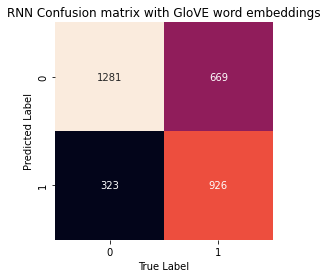
\includegraphics[scale=1]{glove-mat.png}
\end{center}

\begin{center}
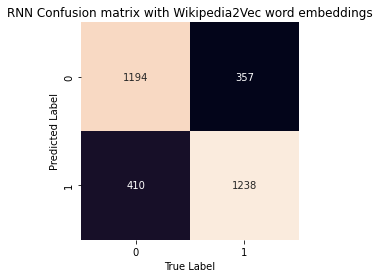
\includegraphics[scale=1]{wiki-mat.png}
\end{center}

\subsubsection{Analysis}
In this experiment, the precisions were similar, with the Wikipedia2Vec model's precision being slightly better. However, the Wikipedia2Vec word embeddings performed much better than the GloVE word embeddings. I think this is because the Wikipedia2Vec model recognized more more words, and missed less words compared to the GloVE model. This could also explaing the slight difference between the precisions of the two models. The difference between the recall values reflect the difference between the number of correctly predicted positive values. In this case, the Wikipedia2Vec model predicted more positives correctly. Similarly, the Wikipedia2Vec model had a greater number of predicted positives than the GloVE model.\\
\\
Comparing the confusion matrices, we can get an idea of how both models performed. Both models had the same number of examples. Therefore, we can compare the number of examples in each cell directly. As mentioned previously, we can see that the number of correctly classified positive is greater for the Wikipedia2Vec model as compared to the GloVE model. Similarly this trend is the same for the number of true negative examples. The GloVE model had significantly more false negatives than false positives. This could have been due to some of the words associated with negative meaning that were not detected using GloVE word embeddings, and were detected using the Wikipedia2Vec word embeddings. Alternatively, this could be due to the fact that the values of the word embeddings were more helpful in that they were able to give more precise and accurate predictions along with a better recall.
\end{document}